\section{Experiment 2 : HTTP}
\subsection{HTTP : The Basic HTTP GET/response interaction}
    \subsubsection*{Experiment Results}
    %
     \vspace{-4mm}
    	\begin{figure}[!h]
    		\centering
    			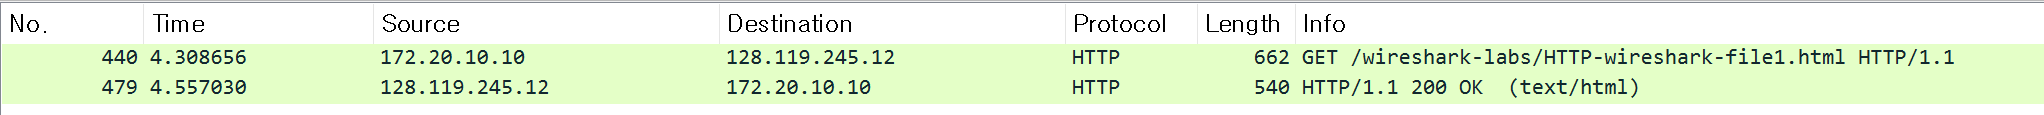
\includegraphics[width=.9\textwidth]{image/week01/2-1.png}
    			\caption{\small Lists of captured packet in the basic HTTP GET/response interaction experiment}
    	\end{figure}
    \vspace{-4mm}  
        \begin{figure}[!h]
            \centering
            \subfloat[662 GET /wireshark-labs/HTTP-wireshark-file1.html HTTP/1.1]{{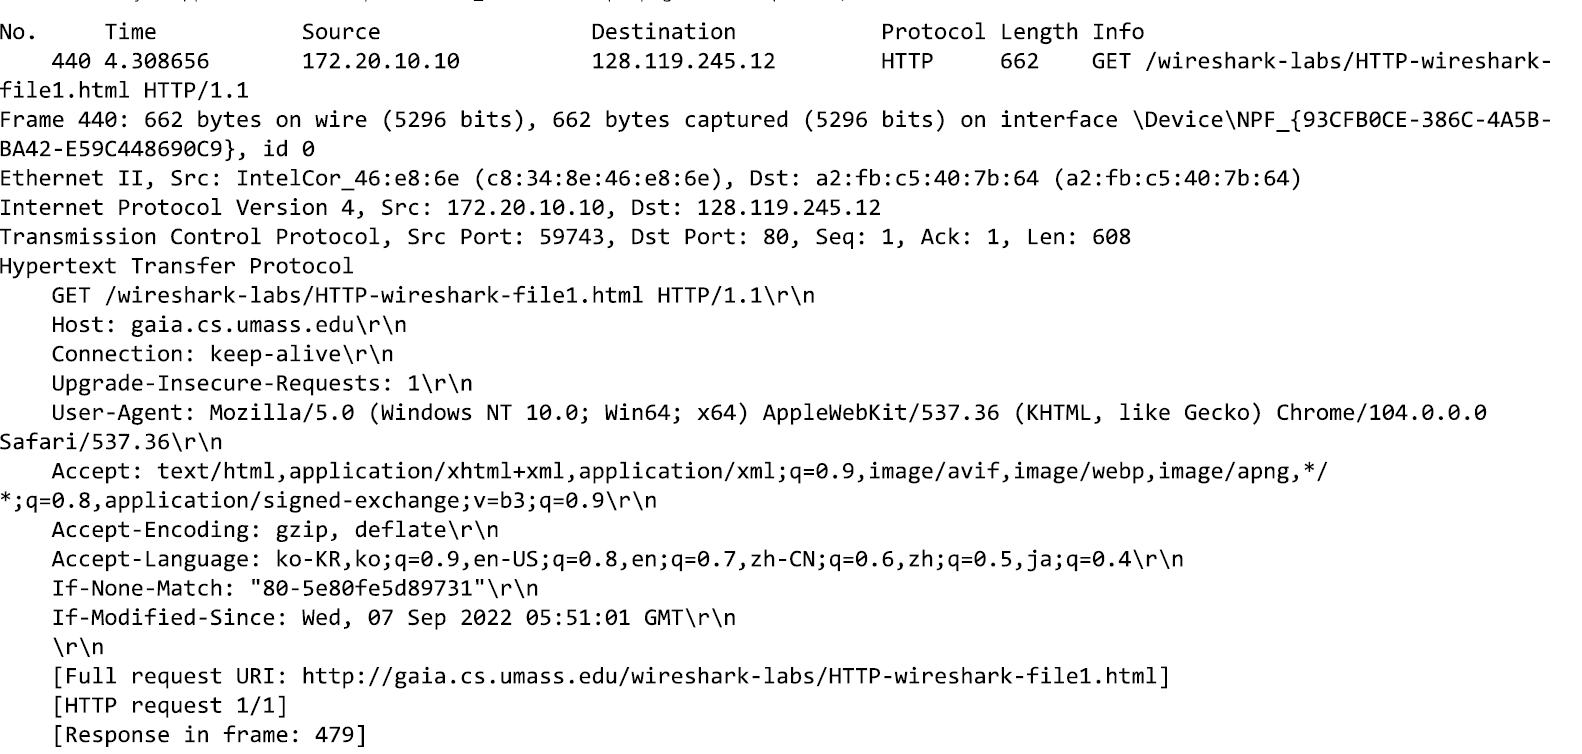
\includegraphics[width=0.9\textwidth ]{image/week01/2-2.png}}}%
            \hfill
            \subfloat[243 HTTP/1.1 304 helloworld.c - adau1761\_init function]{{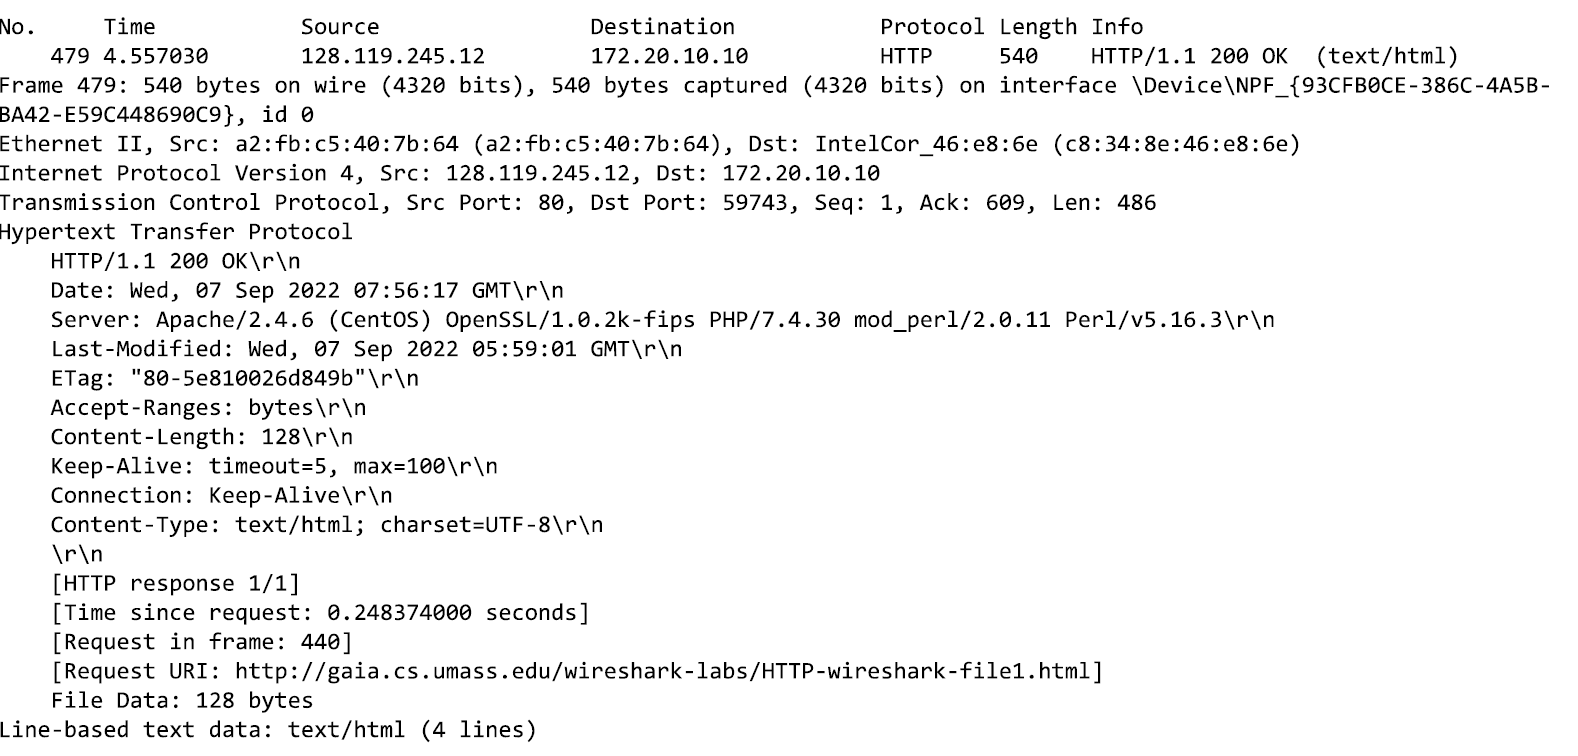
\includegraphics[width=0.9\textwidth ]{image/week01/2-3.png}}}%
            \caption{The Basic HTTP GET/response interaction Experiments results screenshot}
        \end{figure}
    \vspace{-4mm}
    \subsubsection*{Questions}
        \begin{enumerate}[label=\bfseries Problem \arabic*:,leftmargin=*,labelindent=1em]
            \item Is your browser running HTTP version 1.0 or 1.1? What version of HTTP is the server running?\\[0.2mm]
            % 답을 \soln 뒤에 작성하면 됨 
            \soln 
            
            \item What languages (if any) does your browser indicate that it can accept to the server?\\[0.2mm]
            \soln
            
            \item What is the IP address of your computer? Of the gaia.cs.umass.edu server? \\[0.2mm]
            \soln
            
            \item What is the status code returned from the server to your browser?\\[0.2mm]
            \soln 
            
            \item When was the HTML file that you are retrieving last modified at the server? \\[0.2mm]
            \soln
            
            \item How many bytes of content are being returned to your browser? \\[0.2mm]
            \soln
            
            \item By inspecting the raw data in the packet content window, 
            do you see any headers within the data that are not displayed in the packet-listing window?
            If so, name one.\\[0.2mm]
            \soln
            
        \end{enumerate}
\subsection{HTTP : The HTTP CONDITIONAL GET/response interaction}
    \subsubsection*{Experiment Results}
    \begin{figure}[!h]\centering
		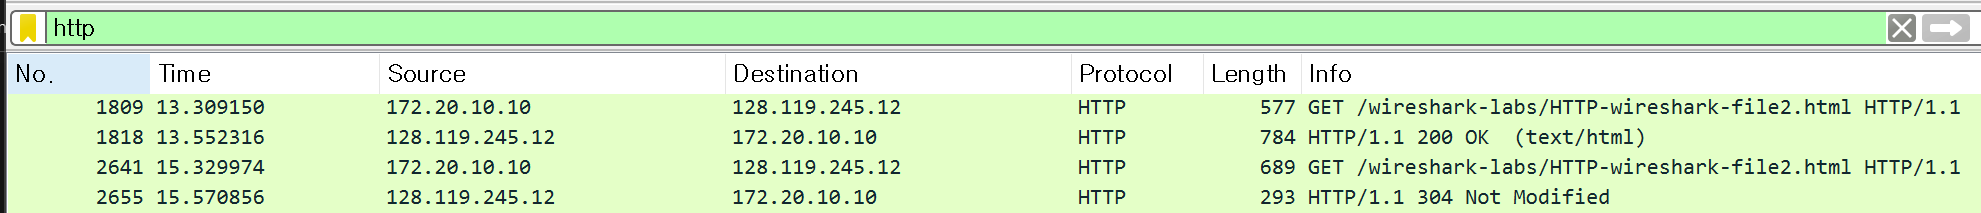
\includegraphics[width=.95\textwidth]{image/week01/2-4.png}
		\caption{\small Lists of captured packet in the HTTP CONDITIONAL GET/response interaction experiment}
	\end{figure}
    \vspace{-4mm}
        \begin{figure}[!h]\centering
    		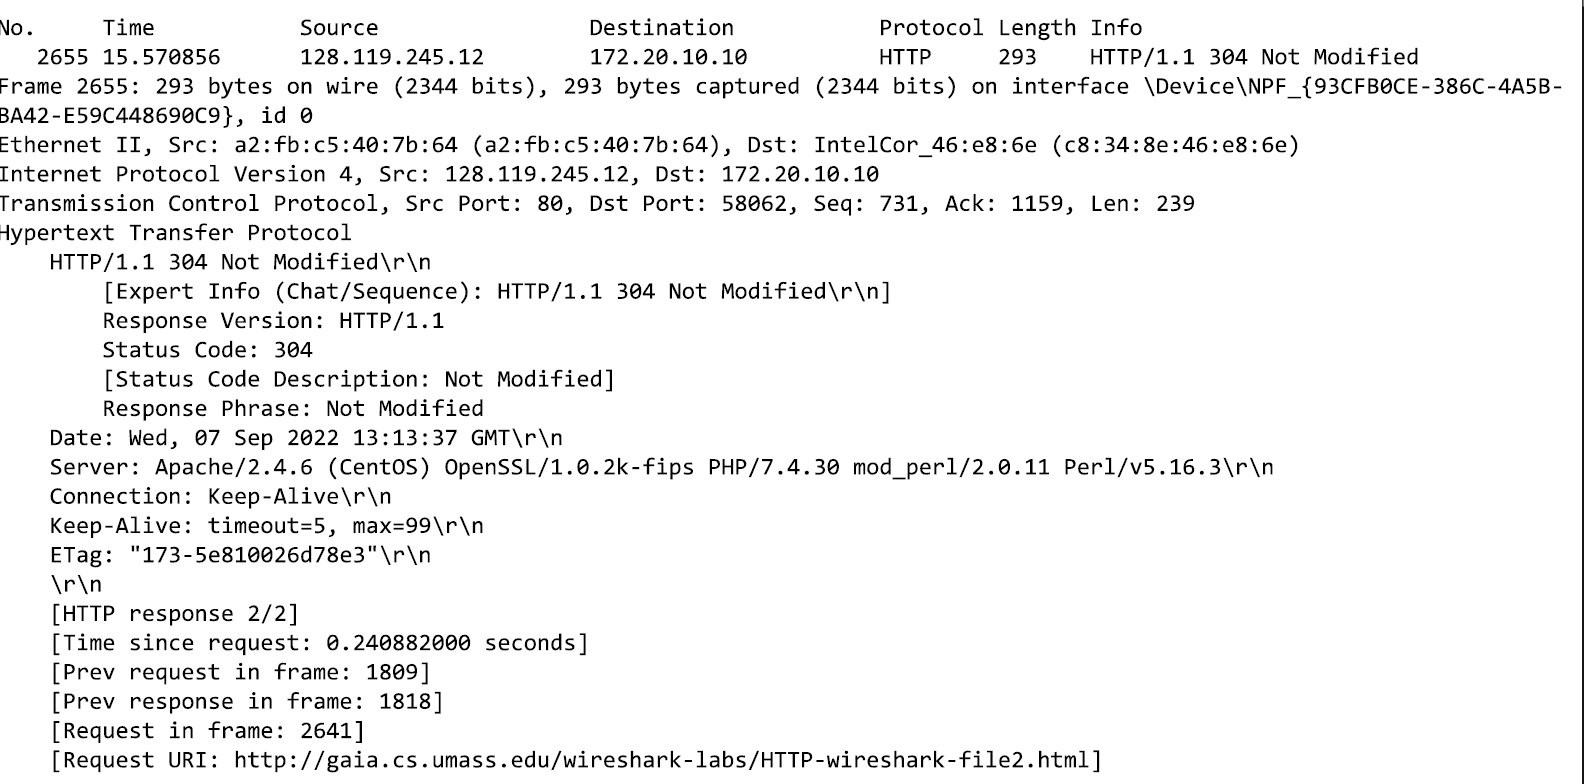
\includegraphics[width=.9\textwidth]{image/week01/2-5.png}
    		\caption*{\small (a) Experiment 2.b : GET wire shark labs wireshark file 2}
        	\end{figure}
        \vspace{-4mm}
\clearpage
        \begin{figure}[!h]\centering
    		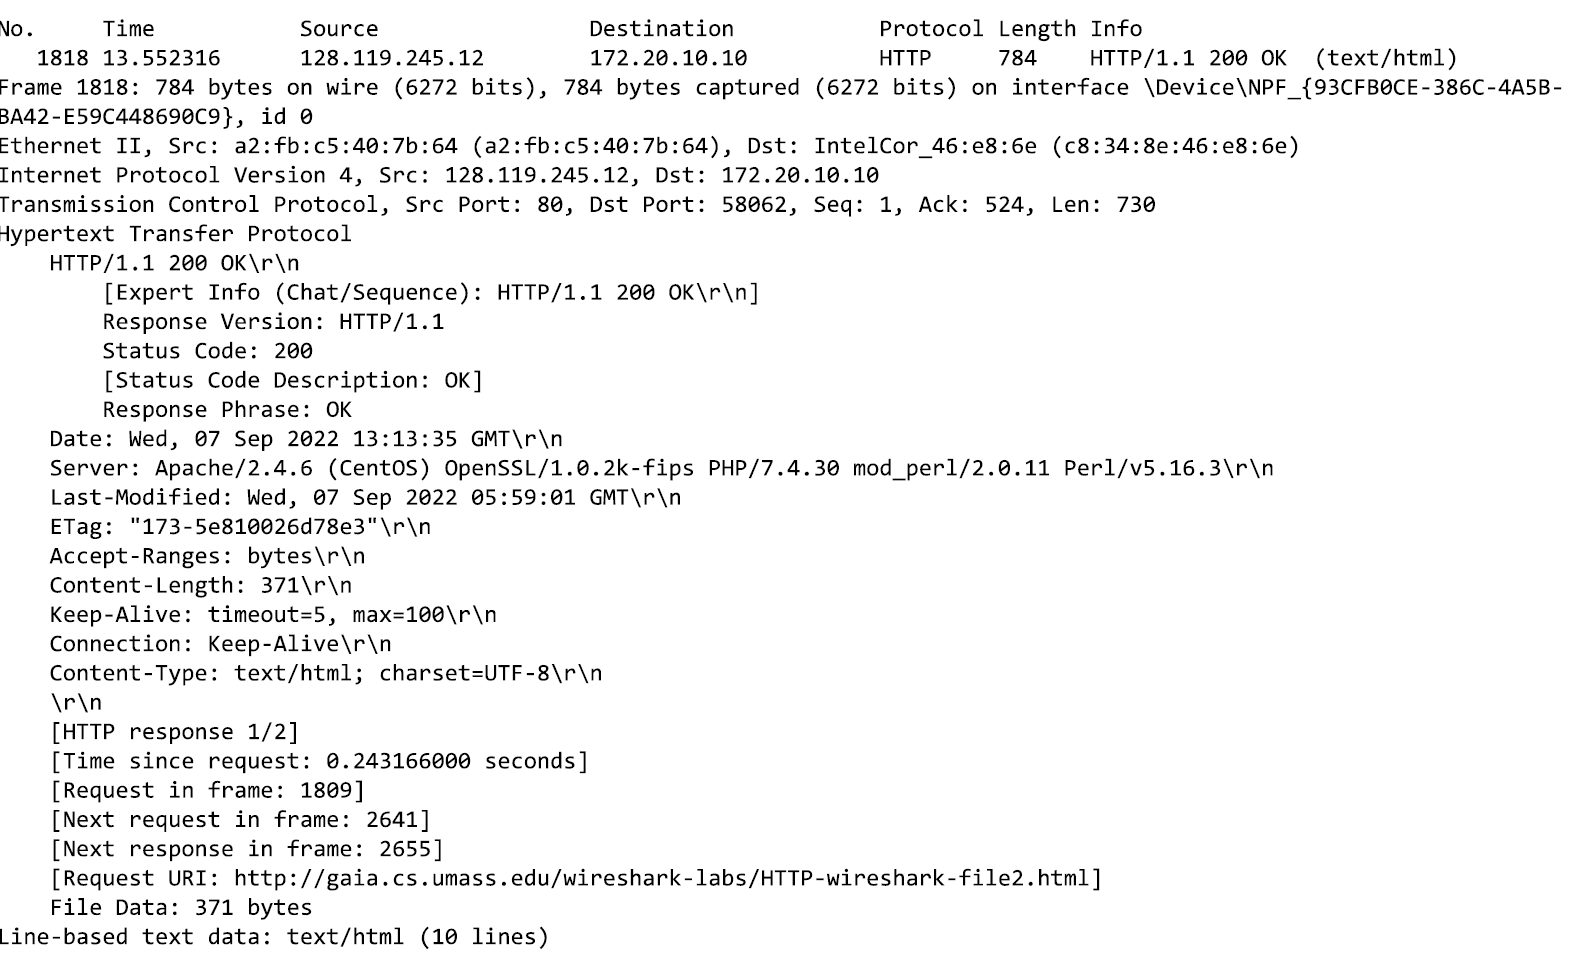
\includegraphics[width=.9\textwidth]{image/week01/2-6.png}
    		\caption*{\small (b) Experiment 2.b : http 1.1 200 OK}
        	\end{figure}
        \vspace{-4mm}
        \begin{figure}[!h]\centering
    		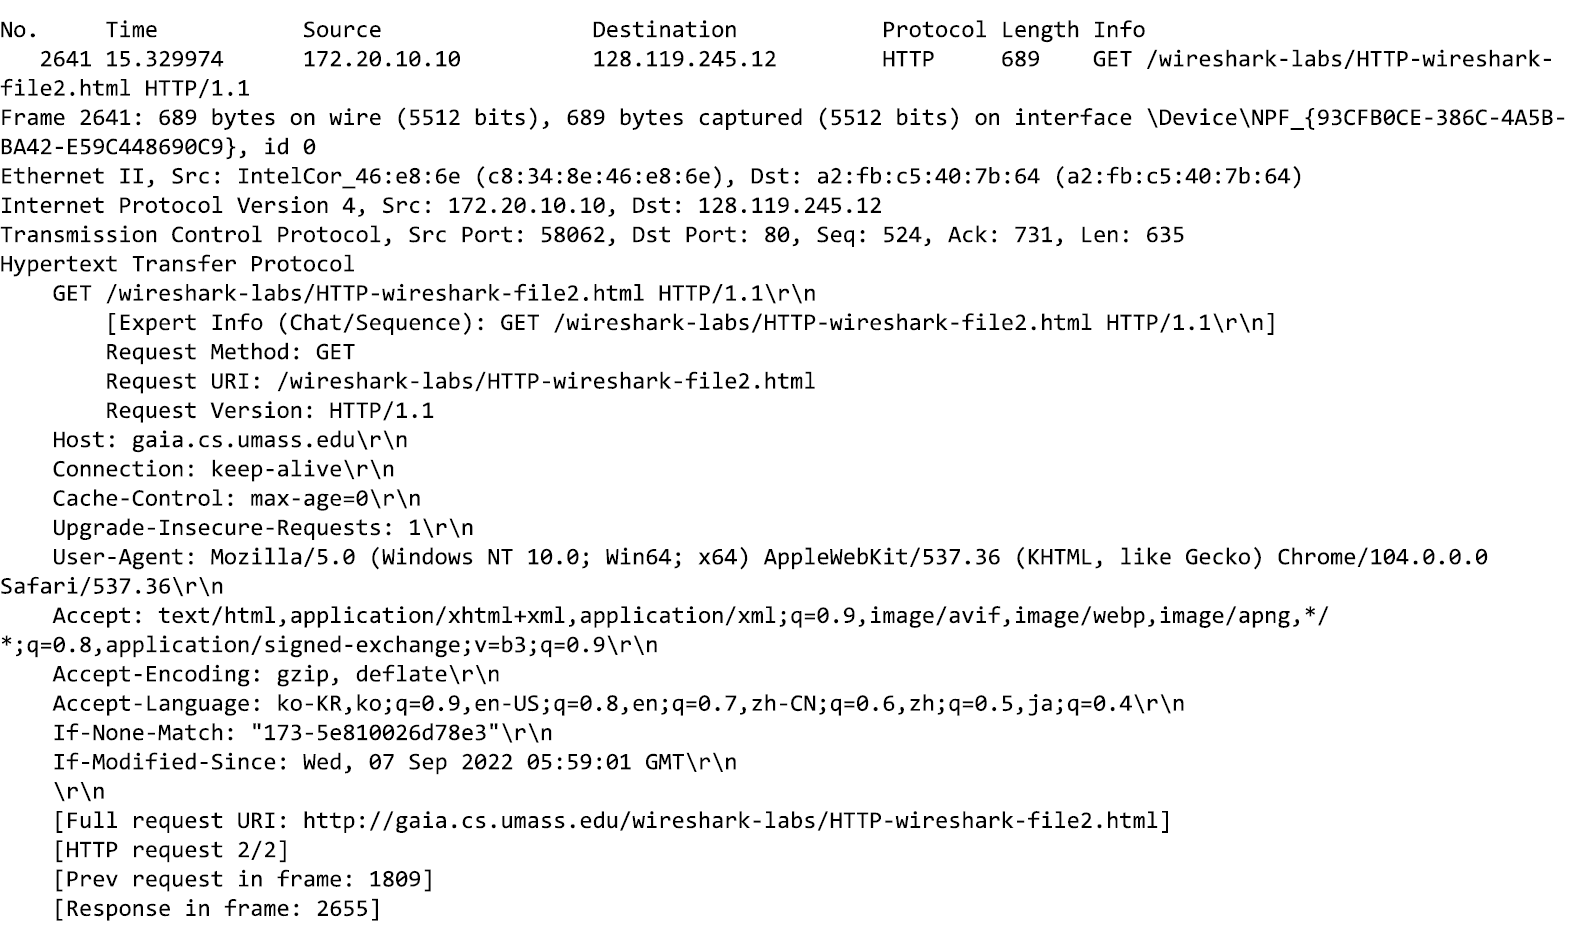
\includegraphics[width=.9\textwidth]{image/week01/2-7.png}
    		\caption*{\small (c) Experiment 2.b : GET wire shark labs wireshark file 2}
        	\end{figure}
        \vspace{-4mm}
        \begin{figure}[!h]\centering
    		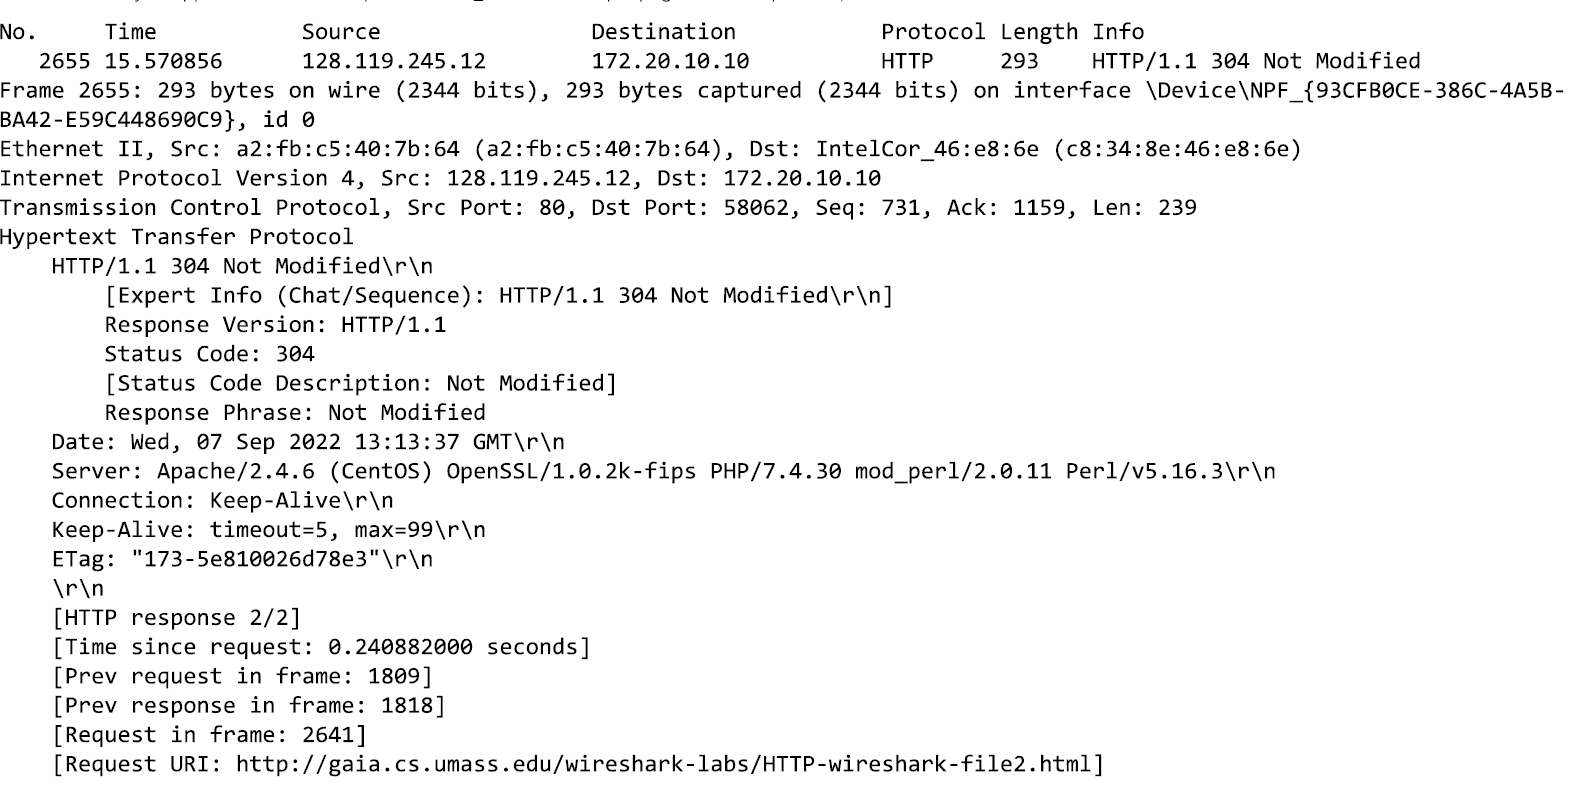
\includegraphics[width=.9\textwidth]{image/week01/2-8.png}
    		\caption*{\small (d) Experiment 2.b : http 1.1 304 not modified }
        	\end{figure}
        \vspace{-4mm}
% 작아서 잘 안보이는데 나중에 그림 파일 수정하면 다시 원래로 바꾸기 

    %     \centering
    %         \subfloat[adau1761 data sheet]{{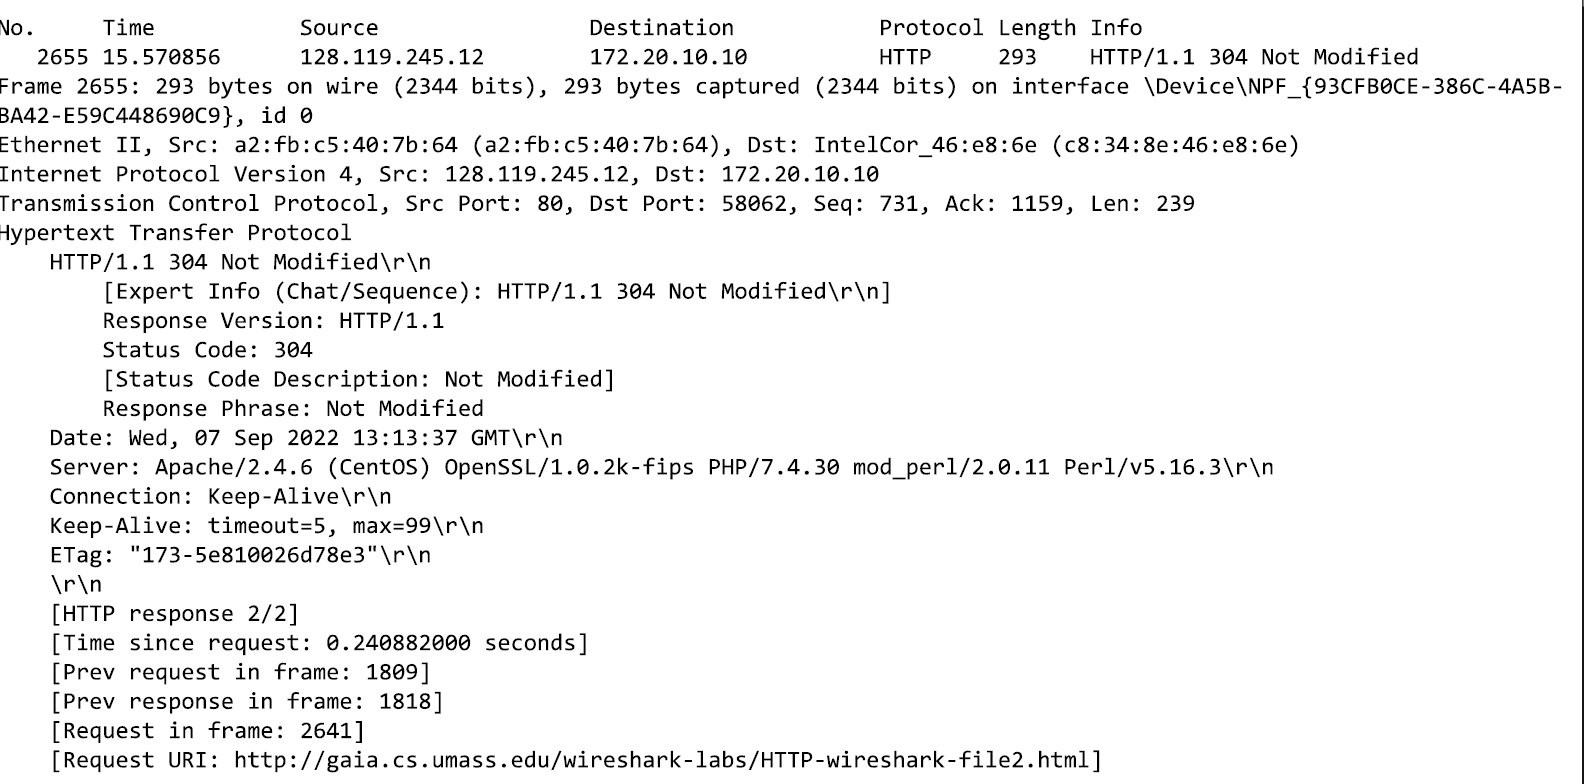
\includegraphics[width=0.75\textwidth ]{image/week01/2-5.png}}}%
    %     \hfill
    %         \subfloat[helloworld.c - adau1761\_init function]{{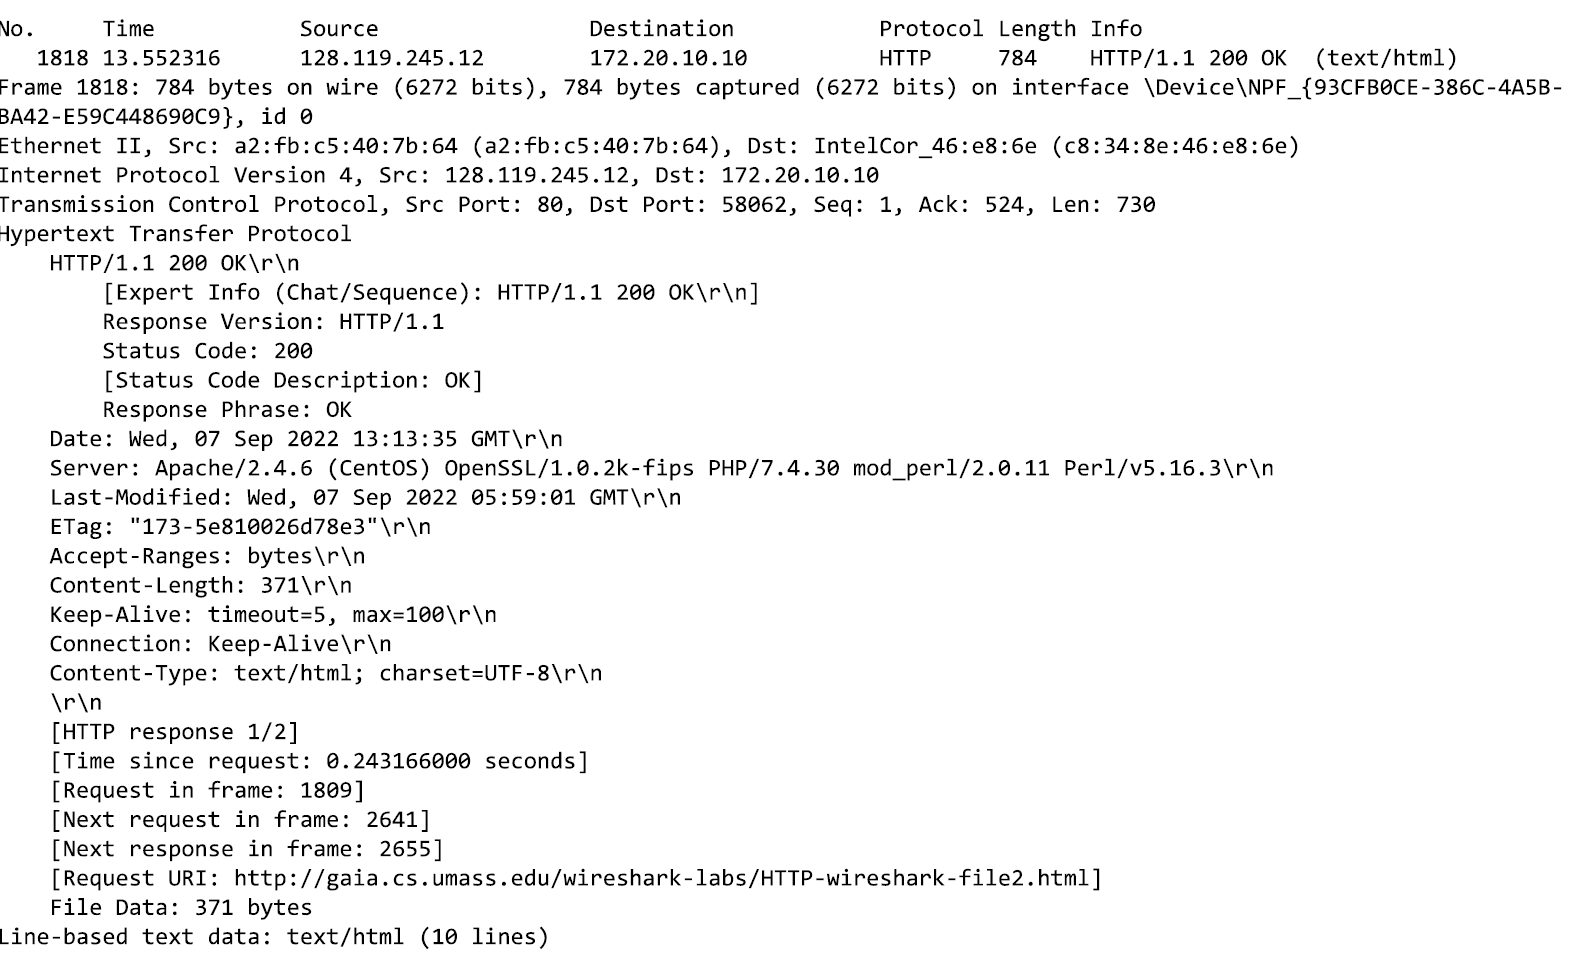
\includegraphics[width=0.75\textwidth ]{image/week01/2-6.png}}}
	   % \hfill
    %         \subfloat[adau1761 data sheet]{{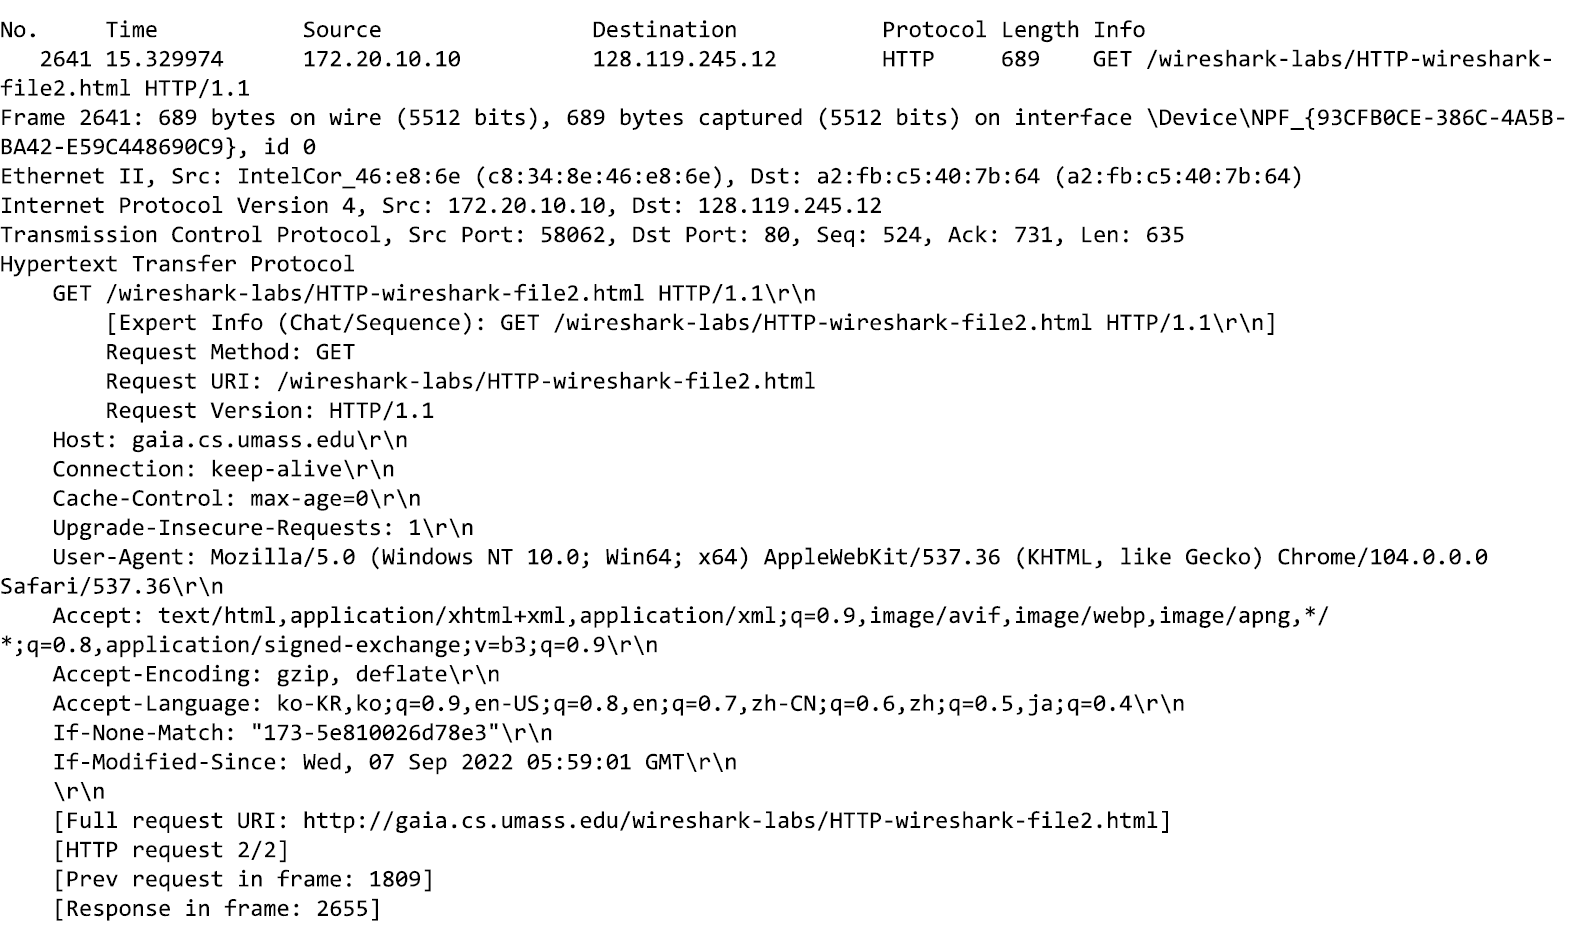
\includegraphics[width=0.75\textwidth ]{image/week01/2-7.png}}}%
    %     \hfill
    %         \subfloat[helloworld.c - adau1761\_init function]{{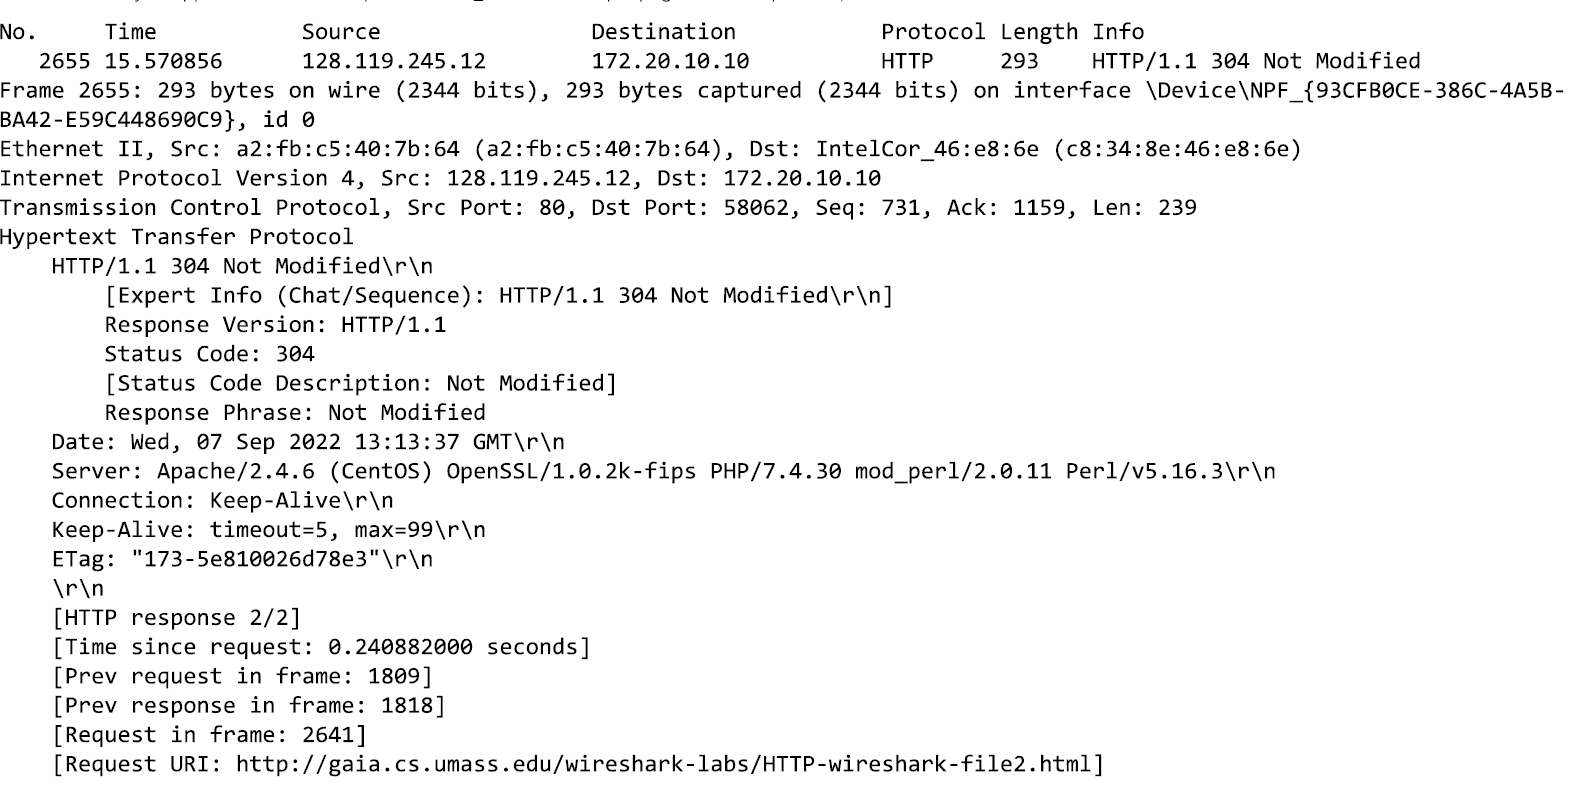
\includegraphics[width=0.75\textwidth ]{image/week01/2-8.png}}}
    %     % \caption{The Basic HTTP GET/response interaction Experiments results screenshot}
    % \end{figure}
    \subsubsection*{Questions}
        \begin{enumerate}[label=\bfseries Problem \arabic*:,leftmargin=*,labelindent=1em]
        \addtocounter{enumi}{7}
            \item Inspect the contents of the first HTTP GET request from your browser to the server.
            Do you see an “IF-MODIFIED-SINCE” line in the HTTP GET? \\[0.2mm]
            \soln
            
            \item Inspect the contents of the server response. Did the server explicitly return 
            the contents of the file? How can you tell? \\[0.2mm]
            \soln
            
            \item Now inspect the contents of the second HTTP GET request from your browser to the server. Do you see an “IF-MODIFIED-SINCE:” line in the HTTP GET? If so, what information follows the “IF-MODIFIED-SINCE:” header?\\[0.2mm]
            \soln
            
            \item What is the HTTP status code and phrase returned from the server in response to this second HTTP GET? Did the server explicitly return the contents of the file? Explain.\\[0.2mm]
            \soln
            
        \end{enumerate}
\subsection{HTTP : Retrieving Long Documents}
    \subsubsection*{Experiment Results}
    	\begin{figure}[!h]\centering
			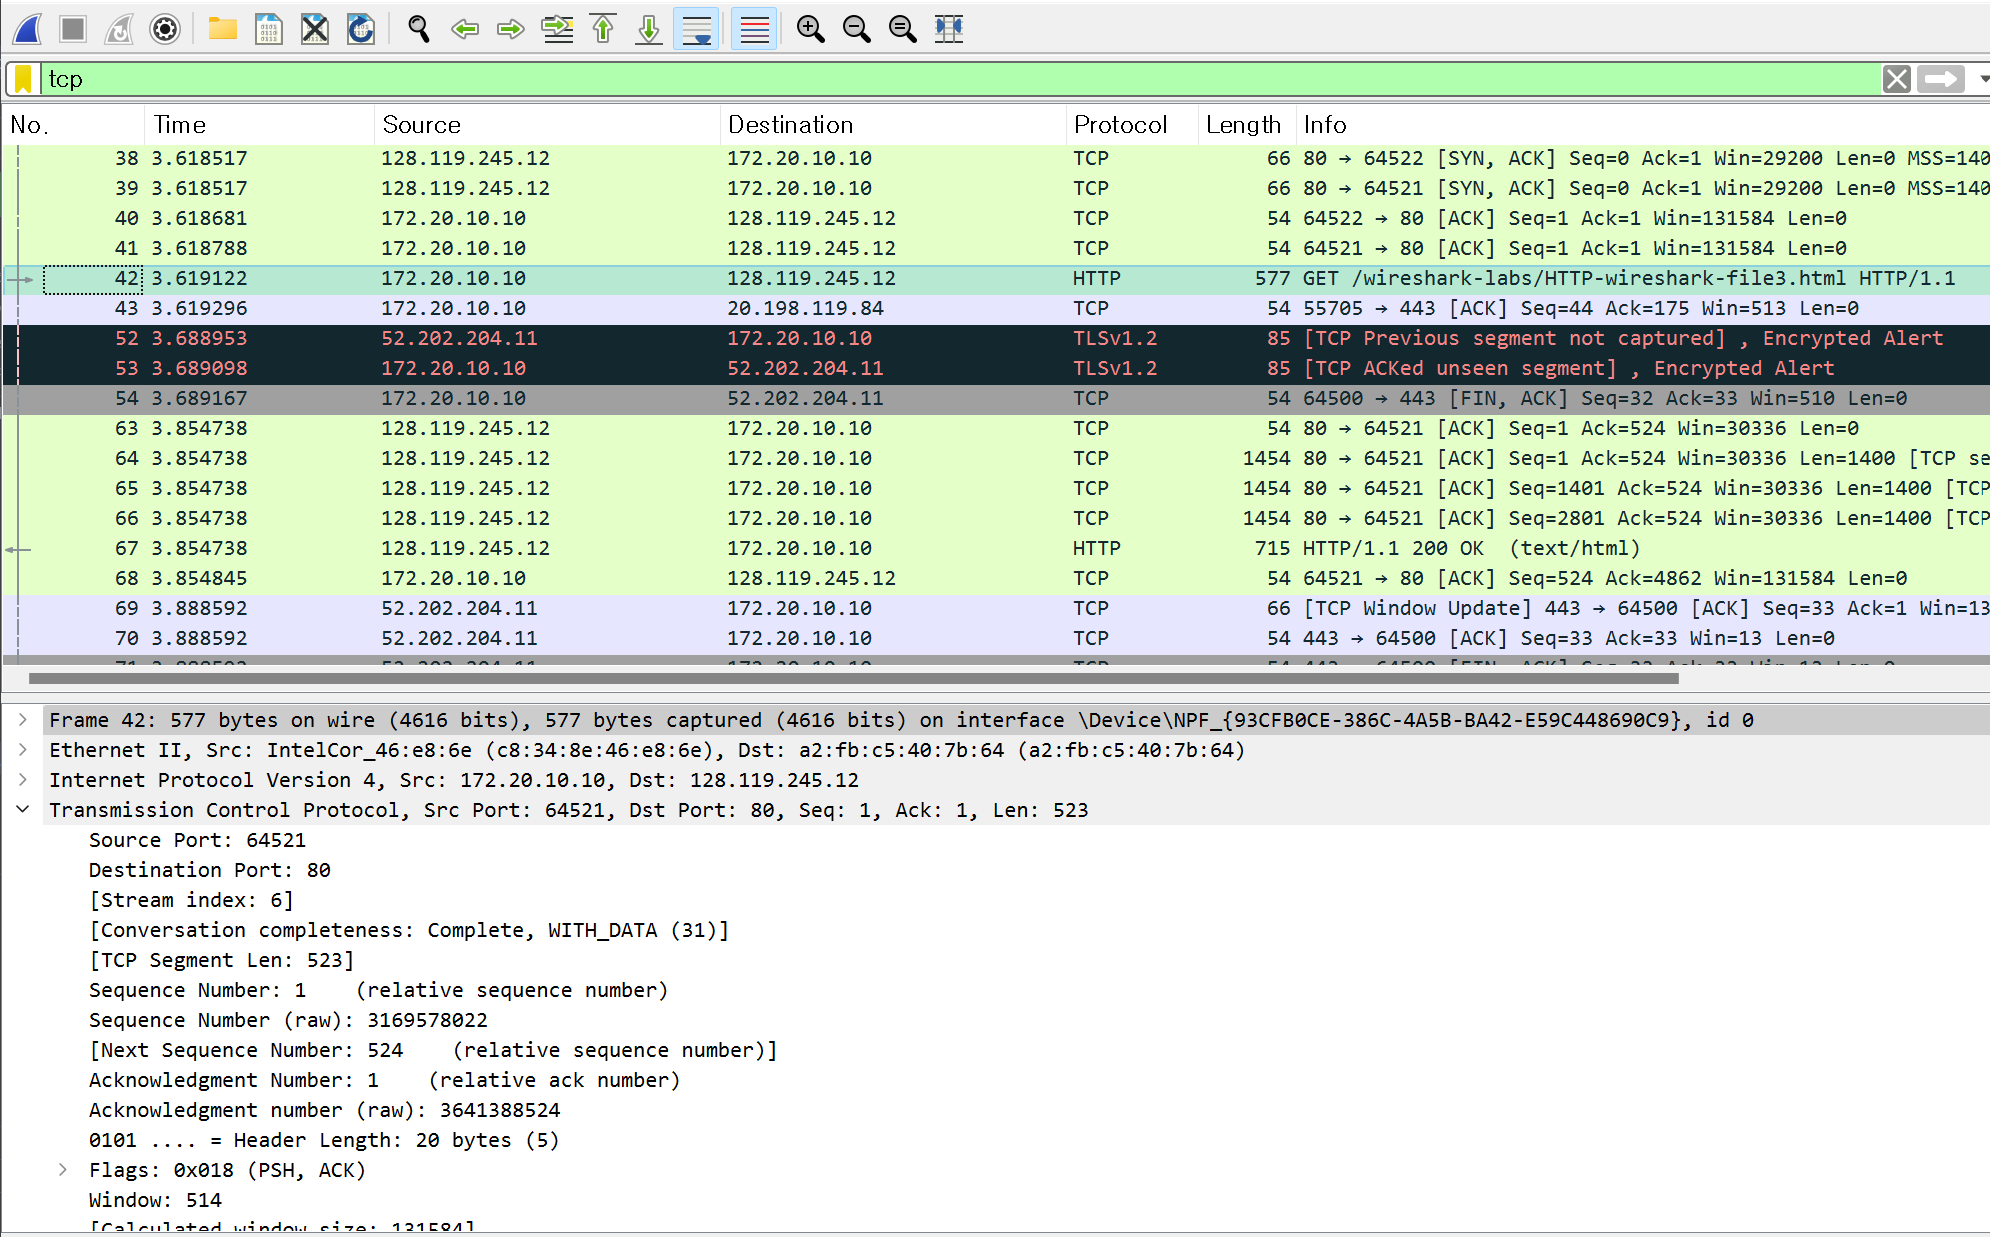
\includegraphics[width=.95\textwidth]{image/week01/2-9.png}
			\caption{Wireshark Screenshot}
    	\end{figure}
    \vspace{-4mm}  
    \subsubsection*{Questions}
        \begin{enumerate}[label=\bfseries Problem \arabic*:,leftmargin=*,labelindent=1em]
        \addtocounter{enumi}{11}
            \item How many HTTP GET request messages did your browser send? \\[0.2mm]
            \soln 1, packet 42
            
            \item Which packet number in the trace contains the status code and phrase associated with the response to the HTTP GET request?\\[0.2mm]
            \soln packet 64 
            
            \item What is the status code and phrase in the response?\\[0.2mm]
            \soln 200 (OK)
            
            \item How many data-containing TCP segments were needed to carry
            the single HTTP response and the text of the Bill of Rights? \\[0.2mm]
            \soln The Packets that of destination adr is "172.20.10.10" in the 
            captured list are packet 63, 64, 65, 66. So the number of 
            data - containing TCP segments are 4.
            
        \end{enumerate}
\newpage